\documentclass{beamer}

\usepackage[francais]{babel}
\usepackage[utf8]{inputenc}
\usepackage[T1]{fontenc}
\usepackage{graphicx}

\mode<presentation>
\usetheme{Darmstadt}

\title{Choisir son clavier}
\author{
  Pierre-Marie de Rodat (PM, \texttt{de-rod\_p})
}
\date{\today}

\begin{document}

\begin{frame}
  \maketitle
\end{frame}

\section*{Introduction}

\begin{frame}{Mais pourquoi~?}
  \begin{itemize}
    \item Difficultés avec les QWERTY sur les postes du campus IONIS~: \pause
      \begin{itemize}
        \item Rapidité \pause
        \item Précision \pause
        \item Jeu de caractères
      \end{itemize}\pause

    \item Le clavier est très utilisé~: important de mieux faire \pause
      \begin{itemize}
        \item Chez soi, en examen et partout ailleurs~! \pause
        \item Changement si possible avant la première année d’ingénieur~!
      \end{itemize}\pause
	\item Vos mains sont précieuses, chérissez-les~!
  \end{itemize}
\end{frame}


\AtBeginSection{
  \begin{frame}
    \tableofcontents[currentsection]
  \end{frame}
}

\section{Vocabulaire}

\begin{frame}{Clavier et keymap}
  \begin{itemize}
    \item Clavier~: dispositif \emph{physique} permettant la saisie. Exemple~: les différents modèles du PIE, le TypeMatrix. \pause
    \item Keymap~: utilisation \emph{logique} du clavier par le système. Exemple~: les dispositions QWERTY, QWERTZ, AZERTY, Dvorak US,  Bépo
  \end{itemize}
\end{frame}



\subsection{Clavier}

\begin{frame}{Anatomie d’un clavier}
  \begin{itemize}
    \item Ensemble de touches disposées sur une «~planche~» \pause
    \item Plusieurs groupes~: pavé alphanumérique, directionnel, numérique, touches de fonction, … \pause
    \item Plusieurs dispositions écrites \pause
    \item Plusieurs paramètres ergonomiques~: taille, éloignement, disposition, profondeur, résistance
  \end{itemize}
\end{frame}

\begin{frame}{Les claviers aujourd’hui}
  \begin{itemize}
    \item Pavé alphanumérique, directionnel, numérique, touches de fonctions (parfois touches multimédia) \pause
    \item Rangées du pavé alphanumérique décalées en escalier («~clavier droit~») \pause
    \item Touches «~Backspace~» et «~Enter~» peu accessibles \pause
  \end{itemize}

  Il existe des alternatives (rarement utilisées)~: \pause
  \begin{itemize}
    \item Claviers compacts~: suppression de pavés (souvent le pavé numérique) \pause
    \item Touches en matrice \pause
    \item «~Backspace~» et «~Enter~» au milieu du pavé alphanumérique
  \end{itemize}
\end{frame}



\subsection{Keymap}

\begin{frame}{Caractéristiques d’une keymap}
  \begin{itemize}
    \item
  \end{itemize}
\end{frame}

\begin{frame}{Les keymaps aujourd’hui}
  \begin{itemize}
    \item De trop nombreuses dispositions existent: colemak, svorak, dvorak(gaucher, droiter, international), bepo, bepo-fr, qwerty, azerty, ...
  \end{itemize}
\end{frame}

\section{Keympas alternatives}

\section{Utilisation}

\section{Le materiel}
\begin{frame}{pourquoi un autre clavier}
    \begin{itemize}
	\item Les claviers standards heritent des lourdeurs du passe: touches en diagonale...
	\item Les claviers matriciels sont beaucoup plus pratiques.
	\pause
	\item TypeMatrix\\
	\begin{figure}
	\centering
	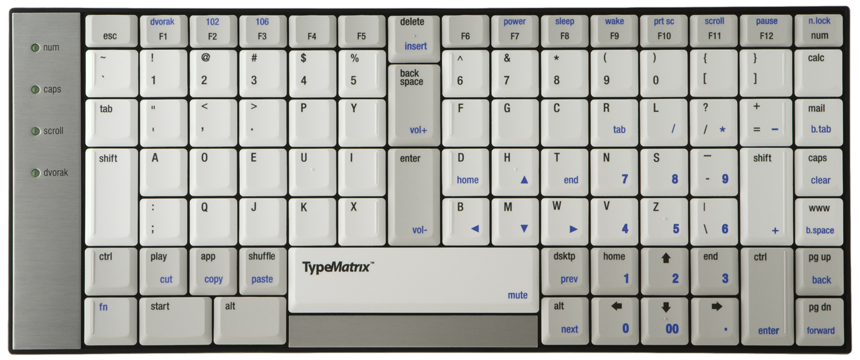
\includegraphics[height=80pt]{images/2030-dvorak.png}
	\end{figure}
    \end{itemize}
\end{frame}
\begin{frame}{materiel - suite}
    \begin{itemize}
	\item Truly-Ergonomics\\
	\begin{figure}
	\centering
	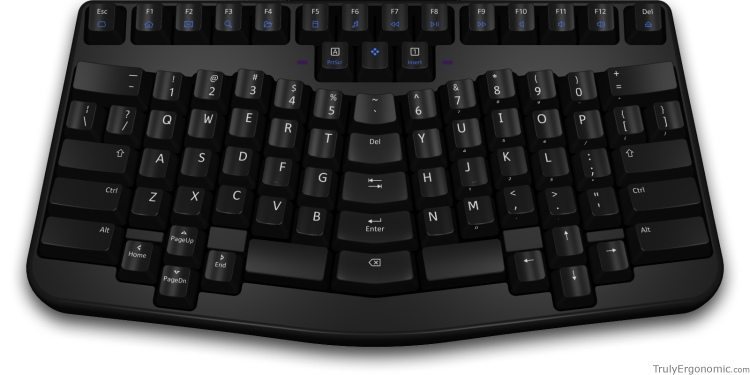
\includegraphics[height=80pt]{images/t_e_keyboard.jpg}
	\end{figure}
	\item Kinesys...
    \end{itemize}
\end{frame}

\section{Les bons logiciels pour apprendre}
\begin{frame}{Les utilitaires}
    \begin{itemize}
	\item GNU typist
	\item le pld bepo (interactif)
    \end{itemize}
\end{frame}

\begin{frame}{Questions}
Soucis, choses pas claires?
\end{frame}


\end{document}
